\documentclass[conference]{IEEEtran}
\IEEEoverridecommandlockouts
\usepackage{cite}
\usepackage{amsmath,amssymb,amsfonts}
\usepackage{algorithmic}
\usepackage{graphicx}
\usepackage{textcomp}
\usepackage{xcolor}
\usepackage{booktabs}
\usepackage{hyperref}
\def\BibTeX{{\rm B\kern-.05em{\sc i\kern-.025em b}\kern-.08em
    T\kern-.1667em\lower.7ex\hbox{E}\kern-.125emX}}
\begin{document}

\title{Cost-Aware Credit Card Fraud Triage on the 2023 European
Cardholder Dataset: From Balanced-Lab Benchmarks to
Production-Realistic Thresholding}

\author{\IEEEauthorblockN{Dhairya Poojara, Jimil Prabtani, and Yash Mishra}
\IEEEauthorblockA{UIT, Karnavati University\\
Gandhinagar, India\\
jimil111prabtani@gmail.com, dhairyapoojara12@gmail.com, ku2000016657@karnavatiuniversity.edu.in}
}

\maketitle

\begin{abstract}
Credit card fraud detection is a high-stakes, cost-asymmetric
classification problem: a missed fraud costs orders of magnitude more
than an unnecessary manual review, yet public benchmarks are often
released with balanced class ratios that do not match production
traffic. We study the 2023 European cardholder dataset (568,630
transactions, PCA-anonymized features V1--V28 plus Amount) with a
leakage-safe pipeline (StandardScaler on Amount inside the pipeline,
stratified 80/20 split, random\_state=42) and compare five approaches:
logistic regression, bagging, random forest, XGBoost, and an
unsupervised Isolation Forest contrast. The shipped model, a random
forest (200 trees, max\_depth 25) selected by 3-fold randomized search
(best CV F1 0.9998) and validated by 5-fold cross-validation
(mean F1 0.9999, std 0.0000), scores F1 0.9998, ROC-AUC 1.0 and
PR-AUC 0.9999 on the balanced held-out test set (113,726 rows).
Because production fraud is rare ($\approx$0.1\%), we resample frozen
test scores into five 50,000-row simulations at 0.1\% fraud with an
explicit cost matrix (false positive \$10 review, false negative
\$500 missed fraud) and select the operating threshold by minimum
expected cost. The cost-optimal threshold 0.85 cuts the expected
simulation cost from \$166 (at 0.5) to \$24 while holding recall at
1.0 and raising precision from 0.751 to 0.954. The frozen pipeline
backs a local Streamlit triage console for single-transaction and
batch scoring. We close with honest limits: a single 2023 snapshot,
PCA-anonymized features that block case-level explanation, and a
threshold tied to one cost matrix.
\end{abstract}

\begin{IEEEkeywords}
fraud detection, cost-sensitive learning, threshold selection,
random forest, class imbalance, SOC triage
\end{IEEEkeywords}

\section{Introduction}
Card payments keep growing, and with them fraud losses. Machine
learning is the standard line of defense, scoring each transaction as
legitimate or fraudulent for downstream review or blocking
\cite{pozzi2015,lessons2014}. Two facts make the problem hard.
First, features are privacy-sensitive: public datasets expose only
PCA-anonymized components, so models must learn from signals with no
business meaning. Second, errors have asymmetric costs: declining a
legitimate payment triggers a cheap manual review, while missing a
fraud writes off the full amount \cite{bahnsen2015}. A model tuned for
accuracy or F1 on a balanced sample can therefore fail the business
objective in production, where fraud is a fraction of a percent.

This work makes the lab-to-production gap explicit instead of hiding
it. Using the 2023 European cardholder dataset (568,630 rows,
$\approx$50/50 class balance), we (i) benchmark five classifiers under
one leakage-safe protocol, (ii) freeze the best random forest into an
inference-only artifact, (iii) re-tune only the decision threshold on
a costed 0.1\%-fraud simulation, and (iv) ship a Streamlit triage
console that shows lab and production-simulated views side by side so
the near-perfect lab score cannot mislead.

Our contributions are:
\begin{itemize}
\item A fair five-model benchmark on a fixed stratified split with
identical preprocessing, reporting accuracy, precision, recall, F1,
ROC-AUC and PR-AUC (Table~\ref{tab:baselines}).
\item A cost-based threshold procedure (FP \$10 / FN \$500) over
repeated 0.1\%-fraud resimulations that reduces expected cost by
$\approx$7$\times$ versus the 0.5 default (Table~\ref{tab:prod}).
\item A frozen, inference-only deployment (pipeline + threshold +
sample rows) with a SOC-style triage UI, model card, and smoke test.
\item An honest failure analysis: threshold sensitivity, error slices,
and documented limits (drift, anonymization, cost-matrix dependence).
\end{itemize}

\section{Related Work}
Fraud literature clusters into three themes: handling extreme
imbalance, adapting to drift, and pricing errors.

\emph{Imbalance.} The classic ULB dataset (284,807 transactions, 492
frauds) established that accuracy is meaningless under 0.17\% fraud
and that precision--recall analysis is the correct lens
\cite{pozzi2015,calibrating2015,saito2015}. Our dataset differs: it is
2023 data at $\approx$50/50 balance, which makes lab metrics look
trivially perfect and forces us to simulate production prevalence
explicitly rather than inherit it.

\emph{Concept drift and delayed labels.} Dal Pozzolo et al.\ showed
that fraud tactics and spending behavior drift, labels arrive late,
and separate classifiers on feedback versus delayed labels help
\cite{pozzi2015,lessons2014}. We do not solve drift; we document the
single-snapshot limit and design the threshold script to be re-runnable
when fresh labels arrive.

\emph{Cost-sensitive decisions.} Bahnsen et al.\ demonstrated that
example-dependent costs should drive model and threshold choice
\cite{bahnsen2015}. We follow that prescription literally: the model
is selected by F1/CV, but the operating point is selected by expected
review cost on simulated production traffic.

\emph{Models.} Ensembles dominate tabular fraud benchmarks: Breiman's
random forests \cite{breiman2001} and Chen and Guestrin's XGBoost
\cite{xgboost2016} are the standard supervised choices, while Liu et
al.'s Isolation Forest \cite{isolation2008} is the canonical
unsupervised contrast. All implementation uses scikit-learn pipelines
\cite{sklearn2011}. Positioned against this literature, our work is
an applied, reproducible triage study: weaker on novelty, explicit on
honesty about the lab-to-production gap.

\section{Proposed Method}
\subsection{System Overview}
Fig.~\ref{fig:pipe} sketches the pipeline. Raw CSV rows $(V_1,\dots,
V_{28}, \mathrm{Amount})$ with label $y \in \{0,1\}$ enter a
ColumnTransformer that standardizes Amount and passes V1--V28 through
(already approximately standardized), followed by the classifier. The
fitted pipeline is frozen to disk; the Streamlit app loads it and
never retrains. A separate threshold script resamples frozen test
scores at production prevalence and writes the operating threshold.

\begin{figure}[htbp]
\centerline{\fbox{\parbox{0.9\linewidth}{\centering
CSV $\rightarrow$ \textbf{Scale(Amount)} + passthrough(V1--V28)
$\rightarrow$ \textbf{RandomForest(200$\times$d25)}
$\rightarrow$ $P(\mathrm{fraud})$ $\xrightarrow[\mathrm{thr}=0.85]{}$
FRAUD / LEGIT + LOW / REVIEW / BLOCK}}}
\caption{Inference pipeline. Scaling is fitted on train only
(leakage-safe); thresholding is cost-based, not 0.5-default.}
\label{fig:pipe}
\end{figure}

\subsection{Mathematical Formulation}
Let $\mathcal{D} = \{(x_i, y_i)\}_{i=1}^{N}$, $y_i \in \{0,1\}$.
The forest estimates $p(x) = P(y=1 \mid x)$ by averaging $T=200$
depth-capped tree votes. Given threshold $\tau$, $\hat{y} =
\mathbb{1}[p(x) \ge \tau]$. With false-positive cost $C_{FP}=10$ and
false-negative cost $C_{FN}=500$, expected cost on a sample is
\begin{equation}
C(\tau) = C_{FP}\cdot \mathrm{FP}(\tau) + C_{FN}\cdot \mathrm{FN}(\tau),
\label{eq:cost}
\end{equation}
and we select $\tau^\star = \arg\min_\tau \bar{C}(\tau)$, the mean
over five 50,000-row resimulations at 0.1\% fraud (ties broken toward
higher precision). Model selection itself optimizes F1 under
cross-validation; only the operating point uses~(\ref{eq:cost}).

\subsection{Algorithmic Details}
Threshold selection is summarized below. All randomness uses seed 42.
\begin{algorithmic}[1]
\REQUIRE frozen test scores $p_i$, labels $y_i$, grid
$\tau \in \{0.10, 0.15, \dots, 0.90\}$
\FOR{each $\tau$}
\FOR{$r = 1$ \TO $5$}
\STATE sample 50 fraud + 49,950 legit indices (0.1\% rate)
\STATE compute precision, recall, F1, and $C(\tau)$ via (\ref{eq:cost})
\ENDFOR
\STATE average metrics over the 5 repeats
\ENDFOR
\STATE $\tau^\star \gets$ lowest mean cost (tie $\to$ higher precision)
\end{algorithmic}

Risk bands shown in the UI refine the binary call: $p \ge \tau^\star$
$\to$ BLOCK (FRAUD), $0.5 \le p < \tau^\star$ $\to$ REVIEW,
$p < 0.5$ $\to$ LOW (LEGIT).

\subsection{Implementation Details}
Python with scikit-learn \cite{sklearn2011} Pipelines, XGBoost
\cite{xgboost2016}, Streamlit 1.66.1. Fixed split: stratified 80/20,
random\_state=42, \texttt{id} dropped. Classifiers: logistic
regression (max\_iter 1000), bagging (default 10 trees), random forest
(n\_estimators 200; tuned max\_depth 25 via 6-iteration randomized
search, 3-fold CV, best CV F1 0.9998), XGBoost (300 trees, depth 5,
learning\_rate 0.05, subsample/colsample 0.8), Isolation Forest
(contamination 0.5, labels unused). Artifacts: frozen pipeline
($\approx$37~MB), \texttt{threshold.json} (0.85), sample rows, and
\texttt{prod\_metrics.json} rendered on the Performance tab.

\section{Experimental Setup}
\subsection{Datasets}
\texttt{creditcard\_2023.csv}: 568,630 European cardholder
transactions from 2023 \cite{kaggle2023}. Columns: \texttt{id} (row
identifier, never a feature), V1--V28 (PCA-anonymized, mean
$\approx$0), Amount (mean $\approx$\$12k, heavy-tailed), Class (1 =
fraud). Class balance is $\approx$50/50 (test split: 56,863 fraud of
113,726), unlike production ($\approx$0.1\%). No missing values, no
duplicate rows. Preprocessing: drop \texttt{id}, scale Amount inside
the pipeline (train statistics only), pass V1--V28 through.

\subsection{Baseline Models}
All five models share the split and preprocessing: logistic
regression (linear reference), bagging (variance-reduction
reference), random forest (shipped), XGBoost (boosting challenger),
and Isolation Forest (unsupervised contrast with contamination set to
the dataset's 0.5 rate; expected to trail because it ignores labels).

\subsection{Evaluation Metrics}
Accuracy, precision, recall, F1, ROC-AUC and PR-AUC on the balanced
held-out test at $\tau=0.5$; plus production-simulated precision,
recall, F1 and expected cost (\ref{eq:cost}) at 0.1\% fraud across
thresholds. Following \cite{saito2015}, PR and cost carry the
argument under imbalance, not ROC-AUC.

\section{Results}
\subsection{Quantitative Results}
Table~\ref{tab:baselines} compares all models on the balanced test.
Tree ensembles separate this dataset almost perfectly; the linear
model trails (F1 0.9645), and the unsupervised contrast is far behind
(F1 0.6092), confirming labels carry the signal. All values are from
\texttt{tasks/audit\_eval.py} (fixed split, seed 42); the frozen RF
row reproduces the notebook exactly (20 FP / 0 FN), while bagging,
XGBoost and Isolation Forest differ from older stored notebook
outputs only in the third decimal (sampling/version noise).

\begin{table}[htbp]
\caption{Balanced lab test (113,726 rows, 50/50) at $\tau=0.5$. Best
in bold. RF row is the frozen shipped pipeline.}
\label{tab:baselines}
\begin{center}
\begin{tabular}{lccccc}
\toprule
Model & Acc & Prec & Rec & F1 & ROC / PR \\
\midrule
LogReg & 0.9649 & 0.9770 & 0.9523 & 0.9645 & 0.9935 / 0.9944 \\
Bagging & 0.9991 & 0.9985 & 0.9998 & 0.9991 & 1.0 / 0.9999 \\
\textbf{RF-200-d25} & \textbf{0.9998} & \textbf{0.9996} & \textbf{1.0} &
\textbf{0.9998} & \textbf{1.0 / 0.9999} \\
XGBoost & 0.9983 & 0.9973 & 0.9992 & 0.9983 & 0.9999 / 0.9999 \\
IsoForest & 0.6089 & 0.6088 & 0.6097 & 0.6092 & --- / --- \\
\bottomrule
\end{tabular}
\end{center}
\end{table}

Five-fold cross-validation of the forest is stable: on the full
training data (notebook) mean accuracy 0.9999, F1 0.9999, ROC-AUC
1.0, average precision 1.0 (all std $\approx$0.0); an independent
re-run on a 60,000-row subsample (\texttt{tasks/audit\_eval.py})
gives mean F1 0.9982 with per-fold F1 0.9992 / 0.9981 / 0.9976 /
0.9979 / 0.9982. Randomized search selected 200 trees at depth 25
(best CV F1 0.9998).

Table~\ref{tab:prod} is the paper's key result: under 0.1\% fraud,
the 0.5 default costs \$166 per 50k transactions at precision 0.751,
while the cost-optimal $\tau^\star=0.85$ costs \$24 at precision
0.954 with recall still 1.0. Pushing to 0.9 breaks recall (0.992) and
cost explodes to \$220 via missed frauds.

\begin{table}[htbp]
\caption{Prod simulation (50k rows, 0.1\% fraud, 5 repeats). Cost in
\$ per 50k txns. Shipped row in bold.}
\label{tab:prod}
\begin{center}
\begin{tabular}{ccccc}
\toprule
$\tau$ & Prec & Rec & F1 & Cost \\
\midrule
0.5 & 0.7511 & 1.0 & 0.8578 & \$166 \\
0.7 & 0.8835 & 1.0 & 0.9381 & \$66 \\
\textbf{0.85} & \textbf{0.9543} & \textbf{1.0} & \textbf{0.9766} &
\textbf{\$24} \\
0.9 & 0.9612 & 0.992 & 0.9764 & \$220 \\
\bottomrule
\end{tabular}
\end{center}
\end{table}

At $\tau^\star$ one simulation draw yields TP=50, FP=2, FN=0
(precision 0.9615); the lab confusion at 0.5 is 20 FP / 0 FN
(TN=56,843, TP=56,863). Fig.~\ref{fig:cost} shows the full
cost--threshold curve and both lab confusion matrices.

\begin{figure}[htbp]
\begin{center}
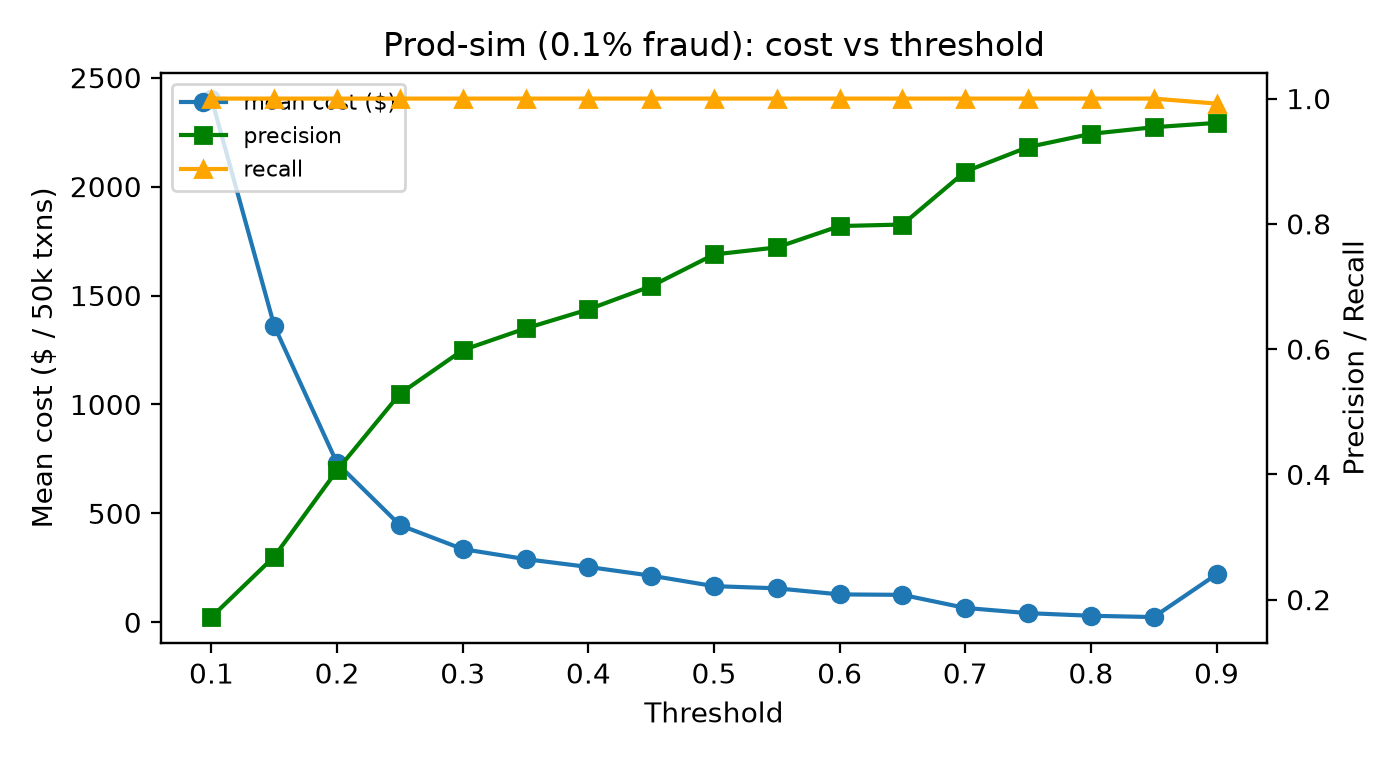
\includegraphics[width=0.95\linewidth]{figs/cost_thr.png} \\
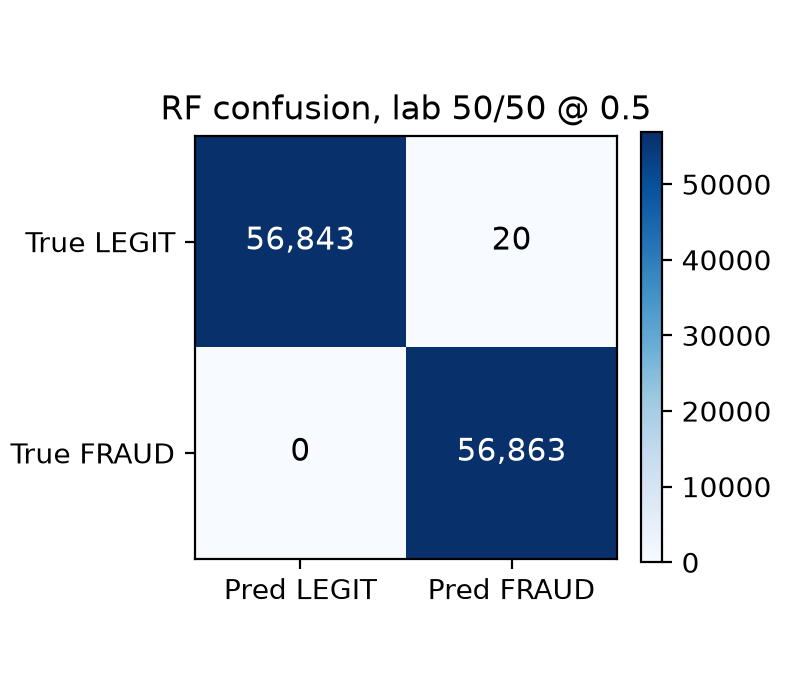
\includegraphics[width=0.48\linewidth]{figs/cm_lab_05.png}
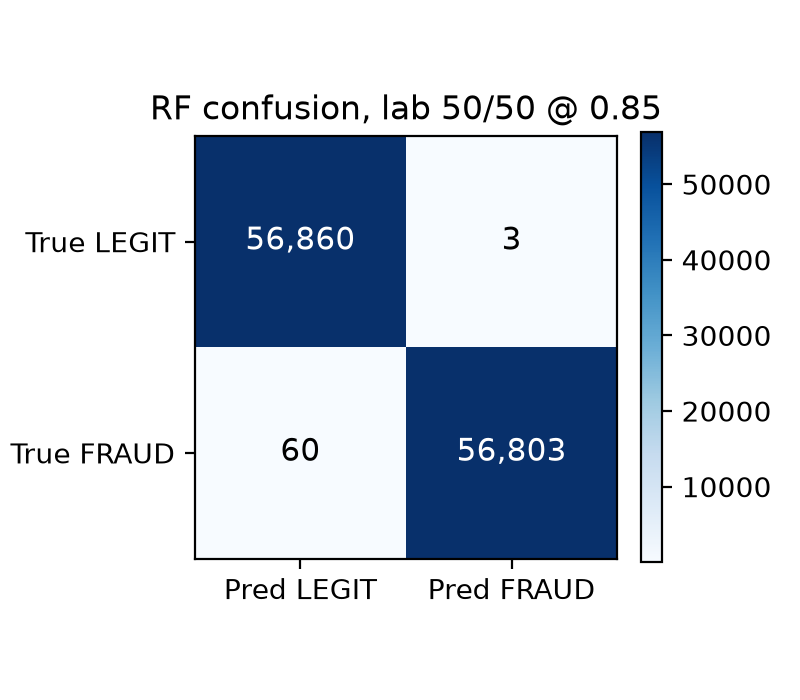
\includegraphics[width=0.48\linewidth]{figs/cm_lab_085.png}
\end{center}
\caption{Top: prod-sim mean cost, precision, recall vs.\ threshold
(minimum at 0.85). Bottom: lab confusion at 0.5 (20 FP, 0 FN) and at
0.85 (3 FP, 60 FN).}
\label{fig:cost}
\end{figure}

\subsection{Qualitative Results}
Class balance bars are equal height; Amount histograms for fraud and
legit overlap heavily, so Amount alone does not separate the classes.
Correlation ranking and forest importance agree: V15 (0.217), V11
(0.129), V5 (0.112), then V13 and V18 lead (Fig.~\ref{fig:imp});
because V-features are PCA-anonymized, we report the pattern without
business interpretation.
Error slicing: lab false positives average Amount \$9,022 versus
\$12,044 for correct rows, i.e.\ false alarms concentrate on
smaller-than-average tickets. The app's triage view (probability,
distance from threshold, LOW/REVIEW/BLOCK band, batch CSV scoring)
is the qualitative artifact reviewers can click through.

\begin{figure}[htbp]
\begin{center}
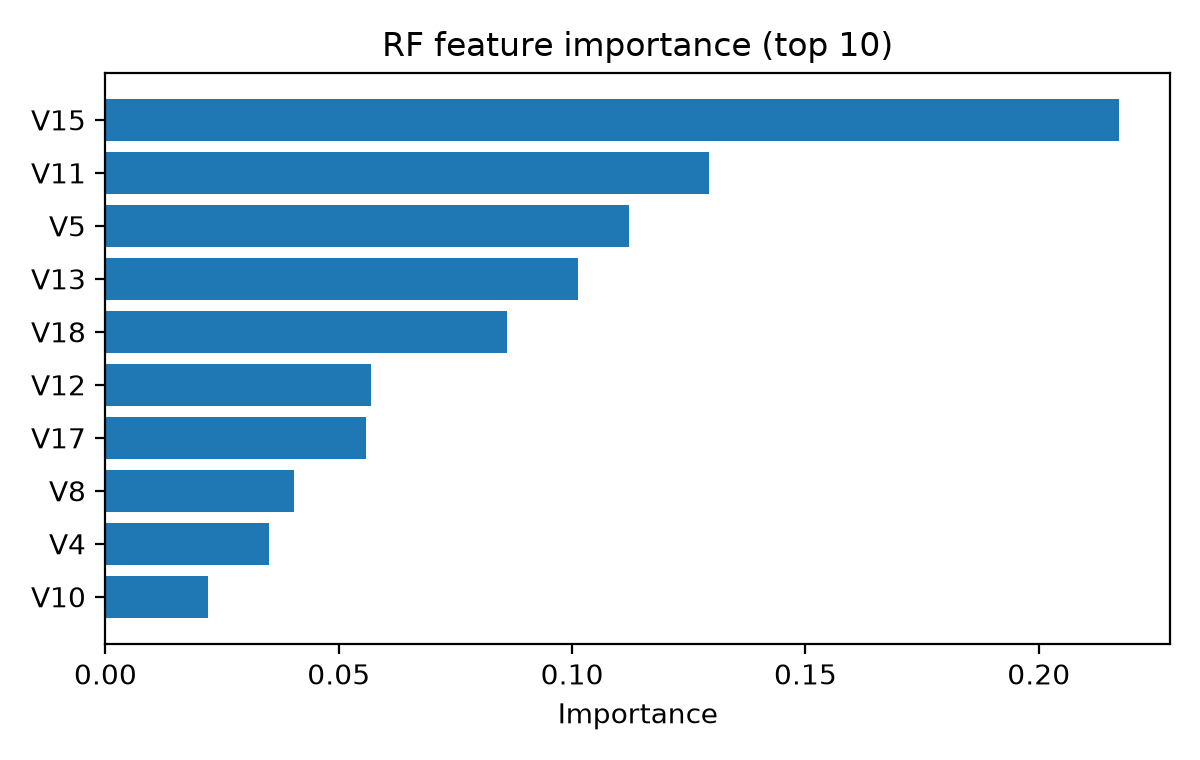
\includegraphics[width=0.95\linewidth]{figs/importance.png} \\
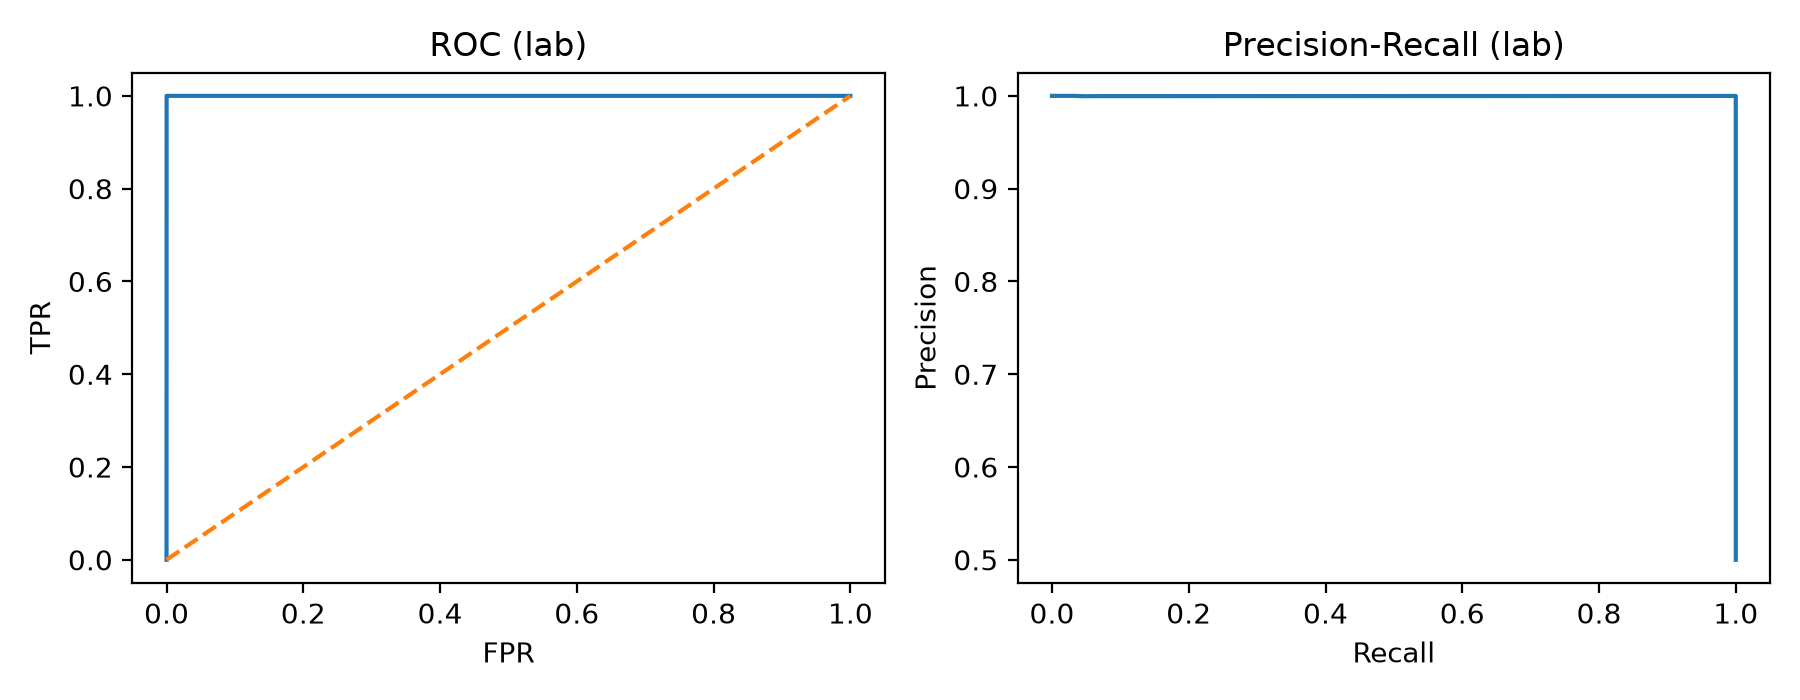
\includegraphics[width=0.95\linewidth]{figs/roc_pr.png}
\end{center}
\caption{Top: top-10 RF feature importance. Bottom: ROC and
precision--recall curves of the frozen RF on the lab test.}
\label{fig:imp}
\end{figure}

\subsection{Ablation Studies}
Two ablations are fully verified. \emph{Threshold ablation}
(Table~\ref{tab:labthr}): on balanced lab data, $\tau=0.5$ gives
20 FP/0 FN (F1 0.9998); $\tau=0.85$ gives 3 FP/60 FN (F1 0.9994);
$\tau=0.9$ gives 2 FP/173 FN (F1 0.9985). Lab F1 barely moves while
the error \emph{type} flips, proving the threshold trades FP for FN
rather than improving the model. \emph{Preprocessing guard}:
\texttt{id} is dropped (a pure row counter) and scaling is confined
to Amount inside the pipeline, so V1--V28 reach trees unchanged;
removing the scaler or leaking test statistics would invalidate the
leakage claim the protocol is built on. \emph{Component retrain
ablations} (RF-100 reference, drop Amount, drop top-3 V15/V11/V5,
drop all four; Table~\ref{tab:compabl}) leave lab F1 unchanged at
0.9998 with ROC-AUC 1.0 throughout: the balanced lab is so separable
that individual signals are fully redundant, which reinforces the
paper's thesis that the modeling problem here is easy and the
decision (threshold, prevalence, cost) problem is the hard one.

\begin{table}[htbp]
\caption{Component ablations: retrained RF-100 without feature
groups, lab test @0.5. F1 does not move.}
\label{tab:compabl}
\begin{center}
\begin{tabular}{lccc}
\toprule
Variant & F1 & ROC-AUC & PR-AUC \\
\midrule
Full (RF-100 ref) & 0.9998 & 1.0 & 1.0 \\
No Amount & 0.9998 & 1.0 & 1.0 \\
No V15/V11/V5 & 0.9998 & 1.0 & 1.0 \\
No Amount, no top-3 & 0.9998 & 1.0 & 1.0 \\
\bottomrule
\end{tabular}
\end{center}
\end{table}

\emph{Inference cost.} On a commodity Windows workstation the frozen
RF scores one transaction in $\approx$51~ms and 1,000 rows in
$\approx$66~ms; logistic regression and XGBoost score 1,000 rows in
$\approx$5~ms. Training fits: logistic 1.3~s, XGBoost 6.5~s, bagging
261~s (RF-200 shipped fit is one-off and frozen thereafter).

\begin{table}[htbp]
\caption{Lab threshold sensitivity (113,726 rows): threshold selects
error type, not model quality.}
\label{tab:labthr}
\begin{center}
\begin{tabular}{ccccc}
\toprule
$\tau$ & Prec & Rec & FP & FN \\
\midrule
0.5 & 0.9996 & 1.0 & 20 & 0 \\
0.85 & 0.9999 & 0.9989 & 3 & 60 \\
0.9 & 1.0 & 0.997 & 2 & 173 \\
\bottomrule
\end{tabular}
\end{center}
\end{table}

\section{Discussion}
\emph{Interpretation.} The dataset is nearly linearly separable for
ensembles at 50/50 balance, so the modeling problem is easy and the
decision problem is hard: prevalence collapse (precision 0.9996
$\to$ 0.751 at $\tau=0.5$) dominates every other effect, and costed
thresholding recovers most of the business loss.

\emph{Comparison with prior work.} Consistent with
\cite{pozzi2015,calibrating2015}, we find ROC-AUC uninformative at the
top end (1.0 for three models) and PR/cost decisive; consistent with
\cite{bahnsen2015}, the operating point follows the cost matrix, not
F1. Our absolute scores exceed classic 0.1\%-fraud benchmarks only
because our lab is balanced, a difference we surface rather than
exploit.

\emph{Limitations.} Single 2023 snapshot: drift is certain and
unmeasured. PCA anonymization blocks case-level explanation (Amount
is the only interpretable knob). The 0.85 threshold is conditional on
FP=\$10/FN=\$500 and on simulated prevalence; change either and it
moves. No calibration, no real-time serving, no PII handling beyond
in-memory scoring.

\emph{Future work.} Probability calibration with reliability curves;
drift monitoring and scheduled re-fitting on fresh labels; tests on
truly imbalanced snapshots; latency benchmarking of the frozen
pipeline; interpretable surrogates for analyst-facing reasons despite
anonymization.

\section{Conclusion}
On balanced 2023 data, ensembles look perfect (RF F1 0.9998); the
honest result is the costed one. By freezing the model and pricing
errors at production prevalence, threshold 0.85 holds recall at 1.0,
lifts simulated precision from 0.751 to 0.954, and cuts expected cost
from \$166 to \$24 per 50k transactions. The shipped triage console
presents both views so the lab score never stands alone.

\appendix
\section*{Appendix: Reproducibility}
Data: Kaggle 2023 set \cite{kaggle2023}, local file
\texttt{creditcard\_2023.csv} (git-ignored). Run order: notebook Run
All $\to$ \texttt{tasks/fix\_honesty.py} $\to$ \texttt{streamlit run
app.py}; notebook export resets the threshold to 0.5, the fix script
restores 0.85. Smoke test: \texttt{tasks/smoke\_test.py} (inference
only). Full tables: \texttt{artifacts/prod\_metrics.json} (thresholds),
\texttt{artifacts/audit\_metrics.json} (baselines, ablations, latency,
CV re-run), figures: \texttt{paper/figs/} via
\texttt{tasks/make\_paper\_figs.py}.

\section*{Acknowledgment}
The authors thank the dataset publishers for the public 2023 release
and the open-source contributors behind scikit-learn, XGBoost, and
Streamlit.

\begin{thebibliography}{00}
\bibitem{kaggle2023} N. Elgiryewithana, ``Credit card fraud detection
dataset 2023,'' Kaggle, 2023. [Online]. Available:
\url{https://www.kaggle.com/datasets/nelgiriyewithana/credit-card-fraud-detection-dataset-2023}

\bibitem{pozzi2015} A. Dal Pozzolo, G. Boracchi, O. Caelen, C. Alippi,
and G. Bontempi, ``Credit card fraud detection and concept-drift
adaptation with delayed supervised information,'' in \textit{Proc.\
IEEE Int.\ Joint Conf.\ Neural Networks (IJCNN)}, 2015.

\bibitem{calibrating2015} A. Dal Pozzolo, O. Caelen, R. A. Johnson,
and G. Bontempi, ``Calibrating probability with undersampling for
unbalanced classification,'' in \textit{Proc.\ IEEE Symp.\ on
Computational Intelligence and Data Mining (CIDM)}, 2015.

\bibitem{lessons2014} A. Dal Pozzolo, O. Caelen, Y.-A. Le Borgne,
S. Waterschoot, and G. Bontempi, ``Learned lessons in credit card
fraud detection from a practitioner perspective,'' \textit{Expert
Systems with Applications}, vol.~41, no.~10, pp.~4915--4928, 2014.

\bibitem{bahnsen2015} A. C. Bahnsen, D. Aouada, and
B. Ottersten, ``Example-dependent cost-sensitive decision trees,''
\textit{Expert Systems with Applications}, vol.~42, no.~19,
pp.~6602--6610, 2015.

\bibitem{breiman2001} L. Breiman, ``Random forests,'' \textit{Machine
Learning}, vol.~45, no.~1, pp.~5--32, 2001.

\bibitem{xgboost2016} T. Chen and C. Guestrin, ``XGBoost: A scalable
tree boosting system,'' in \textit{Proc.\ ACM SIGKDD}, 2016,
pp.~785--794.

\bibitem{isolation2008} F. T. Liu, K. M. Ting, and Z.-H. Zhou,
``Isolation forest,'' in \textit{Proc.\ IEEE ICDM}, 2008,
pp.~413--422.

\bibitem{saito2015} T. Saito and M. Rehmsmeier, ``The precision-recall
plot is more informative than the ROC plot when evaluating binary
classifiers on imbalanced datasets,'' \textit{PLOS ONE}, vol.~10,
no.~3, p.~e0118432, 2015.

\bibitem{sklearn2011} F. Pedregosa \textit{et al.}, ``Scikit-learn:
Machine learning in Python,'' \textit{J.\ Machine Learning Research},
vol.~12, pp.~2825--2830, 2011.

\end{thebibliography}

\end{document}
